\documentclass{article}
% Packages
\usepackage[hidelinks]{hyperref}
\usepackage{graphicx}

\graphicspath{{./images/}}
% Title
\title{Inner Demons\\Game Design}
\author{Josef Větrovský}
\date{11 february}
% Document
\begin{document}
% Titlepage
\maketitle
\thispagestyle{empty}
\cleardoublepage
% Table of contents
\tableofcontents
\thispagestyle{empty}
\cleardoublepage
% Resseting counter
\setcounter{page}{1}
% High level design
\section{High Level Design}\label{high}
    % Rough Script
\subsection{Rough Script}
    A man commits horrible atrocities against his family. After waking from his drunk
    rage, realizing what he's done, he hangs himself. As a punishment for his sins
    he is condemned to wander in his wretched and corrupt mind for the rest of eternity.
    Not knowing where he is, having all kinds of weird feelings, he decides to write them
    on sheets of paper. Broken he sits in a little hut for god knows how long. Unable
    to do anything. Desoriented, confused, sad, angry and yet he feels nothing.
    One time he finds the strength to get up and wanders off to the never ending night.

    The game begins here... or does it? The player finds himself in the body of this
    spoiled, though now hopeless, man. With only one way to go, and that is forward,
    he walks through the strange and sad environment of our character's mind.
    
    As we progress, we find papers written by a certain somebody. They are the main way to reveal the story of
    this game. They also become increasingly confusing and strange. So does the environment.

    Later in the game, the player also acquires a gun with which he can fight the demons
    inside the mind of our main character.

    Going through this unpleasant place, we can truly see, who this man really was.
    The demons get stronger as the player progresses through the game.
    At the end, there is a boss fight. The Devil within our main character. If the player
    manages to destroy him, he will be greeted with the end screen. After the end screen
    ends, the player wakes up back at the beggining.

    The point of the game is, that some sins are unforgettable. Redeeming yourself in
    this game is not an option. One way or another, the player will end up at the begging again.

    Very important piece of this game is the music. It sets the mood of the whole game.
    % Setting Of The Story
\subsection{Setting Of The Story}
Sad western-like environment. Naked and rotten trees, old buildings, overgrown fields.
Neverending darkness, crows. Lots of blood, cemeteries, empty towns. Everything gets
worse as the games progresses. 
    % Target Player Type 
\subsection{Target Player Type}
More patient players, that like atmosphere and would want to uncover the secrets of the
game's story. This game does not offer much of action, player should be aware of that,
although there are a few elements of combat. This game is made for players, who want
to dive into a deep and scientifically meticulous story. They should
enjoy the minimalistic 2D combat and artwork.
    % Core Game Mechanics
\subsection{Core Game Mechanincs}
There are not many special mechanics in this game. It is mainly about storytelling and
atmosphere. The is a simple shooting mechanic. Enemies are not especially interesting
and they are not even meant to. Everything is 2D, so the graphics are also very simple.
So walk, run, jump and shoot.
    % High Lights
\subsection{High Lights}
This game is innovative in the way of telling its interesting story. Because the player
does not know what is happening until the very end. He reveals the story slowly throughout
the entire game. This forces the player to keep going. The implementation of some simple
action in form of shooting enemies is a way of entertaining the player. It also fits the
setting.

This game also has a moral lesson in it. There is not a single happy thing in this game,
not a single spark of joy or hope. The fate of the main character is decided and the player can do nothing
to change it. Which makes the entire run quite pointless. And this is also a moral lesson.

This game should also be great in setting the atmosphere with its carefully picked
music. Just listen to it...
\cleardoublepage
% Game Design
\section{Game Design}
    % Script
\subsection{Script}
An unnamed man kills his family in a fit of rage. After realizing, what he's done, he hangs himself. For his sins, he is condemned to wander his own rotten mind for the rest of eternity.

After a long time of confused wailing, unable to do anything, just lying in a small old hut, he decides to take action and cleanse his own mind. He wanders into the darkness, stopping only to write letters, just to keep himself sane, knowing that no one will ever read them. Along the way he finds a gun and uses it to fight off the demons in his mind. The environment gets darker and more wicked as he progresses and his sanity diminishes more and more, which can be seen in his letters.

In the end, the puts up a fight with the devil within him. After defeating him, he faints, only to find himself back at the beginning, with his memory wiped, going on the same journey, he just completed, because even if he wanted to, he cannot change his fate. He will stay trapped in his wicked mind forever.
    % Locations
\subsection{Locations}
The whole map is just one location. It changes vibe as you progress through the game.

You start in an overwrown grain fields with a small hut a an old tree nearby. The places will
look similar for some time. After a while it gets darker and you go deeper through mines.

The whole western themed environment is sad, overgrown and dark.

On strategic point in the game, letters are placed.
    % Level Design
\subsection{Level Design}
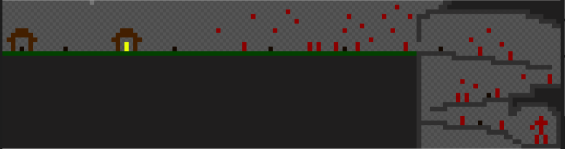
\includegraphics{level_design.png}\\
Note that this is just an outline of the real map.\\
\\
One pixel wide - red - above ground - flying demons\\
Two pixels wide - red - on the ground - normal demons\\
One pixel wide - dark brown - on the ground - letters\\
Two pixels wide - yellow - on the ground - gun\\
Big red thing at the end - the devil within
    % Dialogs
\subsection{Dialogs}
There are no dialogs in this game. You are completely alone.
    % Technical Design
\subsection{Technical Design}
\textbf{Health:}\\
Player health - 3 HP\\
Normal demon - 3 HP\\
Flying demon - 1 HP\\
The devil within - 20 HP\\
\\
\textbf{Damage:}\\
Gun damage - 1 HP\\
\\
\textbf{Number of letters:} 8

    % User Interface
\subsection{User Interface}
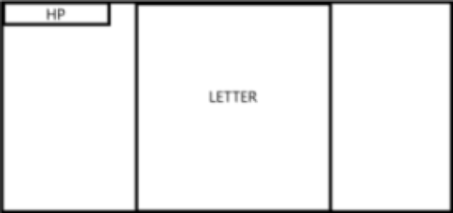
\includegraphics{HUD}\\
HP bar is present at all times.\\
When letters are opened, they can be viewed at the center of the screen as shown in the picture.
    % Controls Design
\subsection{Controls Design}
Movement - A and D keys\\
Jump - SPACE\\
Shoot - LEFT CLICK where you want to shoot\\
Interact - E key
    % Sound
\subsection{Sound}
Few songs from various interprets. Slow and atmospheric\\
Ambient sounds
\end{document}